\documentclass[12pt]{article}
\usepackage[margin=2.5cm]{geometry}
\usepackage{enumerate}
\usepackage{amsfonts}
\usepackage{amsmath}
\usepackage{fancyhdr}
\usepackage{amsmath}
\usepackage{amssymb}
\usepackage{amsthm}
\usepackage{mdframed}
\usepackage{graphicx}
\usepackage{subcaption}
\usepackage{adjustbox}
\usepackage{listings}
\usepackage{xcolor}
\usepackage{courier}
\usepackage[utf]{kotex}
\usepackage{hyperref}
\usepackage{soul}

\definecolor{codegreen}{rgb}{0,0.6,0}
\definecolor{codegray}{rgb}{0.5,0.5,0.5}
\definecolor{codepurple}{rgb}{0.58,0,0.82}
\definecolor{backcolour}{rgb}{0.95,0.95,0.92}

\lstdefinestyle{mystyle}{
    backgroundcolor=\color{backcolour},
    commentstyle=\color{codegreen},
    keywordstyle=\color{magenta},
    numberstyle=\tiny\color{codegray},
    stringstyle=\color{codepurple},
    basicstyle=\ttfamily\footnotesize,
    breakatwhitespace=false,
    breaklines=true,
    captionpos=b,
    keepspaces=true,
    numbers=left,
    numbersep=5pt,
    showspaces=false,
    showstringspaces=false,
    showtabs=false,
    tabsize=1
}

\lstset{style=mystyle}

\pagestyle{fancy}
\renewcommand{\headrulewidth}{0.4pt}
\lhead{CSC 369}
\rhead{Midterm 2 Solution}

\begin{document}
\title{CSC 369 Midterm 2 Solution}

\bigskip

\begin{enumerate}[1.]
    \item

    \begin{enumerate}[a)]
        \item False
        \item True
        \item True
        \item True
        \item True
        \item False
    \end{enumerate}

    \bigskip

    \begin{mdframed}
    \underline{\textbf{Correct Solution}}

    \bigskip

    \begin{enumerate}[a)]
        \item False
        \item True
        \item True
        \item \color{red}False\color{black}

        \bigskip

        \color{red}(I am not too sure. But this may be due to the system setting up
        limited direct execution (baby proofing the CPU) before resuming the program)\color{black}

        \bigskip
        \item \color{red}False\color{black}

        \bigskip

        \color{red}(I am not too sure. But this may be because the lock spins using CPU
        cycle until spinlock is available for the process. Using this,
        the process may be in running state and not the blocked state)\color{black}

        \bigskip

        \item False
    \end{enumerate}
    \end{mdframed}

    \bigskip

    \underline{\textbf{Notes}}

    \bigskip

    \begin{itemize}
        \item \textbf{User Mode}

        \begin{itemize}
            \item Is restricted
            \item Executing code has no ability to \textit{directly} access
            hardware or reference memory $^{[1]}$
            \item Crashes are always recoverable $^{[1]}$
            \item Is where most of the code on our computer / applications are executed $^{[3]}$
        \end{itemize}

        \item \textbf{Kernel Mode}
        \begin{itemize}
            \item Is previleged (non-restricted)
            \item Executing code has complete and unrestricted access to the underlying hardware $^{[3]}$
            \item Is generally reserved for the lowest-level, most trusted functions of the operating
            system $^{[1]}$
            \item Is fatal to crash; it will halt the entire PC (i.e the blue screen of death) $^{[3]}$
        \end{itemize}

        \item \textbf{Interrupt}

        \begin{itemize}
            \item Are signals sent to the CPU by external devices, normally I/O devices. $^{[2]}$
            \item Tells the CPU to stop its current activities and execute the appropriate part of the operating system (\textbf{Interrupt Handler}). $^{[2]}$
            \item Has three different types $^{[2]}$

            \begin{enumerate}[1)]
                \item \textbf{Hardware Interupts}

                \begin{itemize}
                    \item Are generated by hardware devices to signal that they need some attention from the OS.
                    \item May be due to receiving some data

                    \bigskip

                    \underline{\textbf{Examples}}

                    \bigskip

                    \begin{itemize}
                        \item Keystrokes on the keyboard
                        \item Receiving data on the ethernet card
                    \end{itemize}

                    \bigskip

                    \item May be due to completing a task which the operating system previous requested

                    \bigskip

                    \underline{\textbf{Examples}}

                    \bigskip

                    Transfering data between the hard drive and memory
                \end{itemize}

                \bigskip

                \item \textbf{Software Interupts}

                \bigskip

                \begin{itemize}
                    \item Are generated by programs when a system call is requested
                \end{itemize}

                \bigskip

                \item \textbf{Traps}

                \bigskip

                \begin{itemize}
                    \item Are generated by the CPU itself
                    \item Indicate that some error or condition occured for which assistance from the operating system is needed
                \end{itemize}

                \bigskip
            \end{enumerate}
        \end{itemize}

        \item \textbf{Content Switch}

        \begin{itemize}
            \item Is switching from running a user level process to the OS kernel and often
            to other user processes before the current process is resumed
            \item Happens during a timer interrupt or system call
            \item Saves the following states for a process during a context switch
            \begin{itemize}
                \item Stack Pointer
                \item Program Counter
                \item User Registers
                \item Kernel State
            \end{itemize}
            \item May hinder performance
        \end{itemize}

        \item \textbf{System Call}

        \bigskip

        \underline{\textbf{Example}}

        \begin{itemize}
            \item \texttt{yield()}
            \begin{itemize}
                \item Is a system call
                \item Causes the calling thread to relinquish the CPU
                \item Places the current thread at the end of the run queue
                \item Schedules another thread to run
            \end{itemize}
        \end{itemize}

        \item \textbf{Thread}

        \begin{itemize}
            \item Is a lightweight process that can be managed independently by a schdeduler $^{[4]}$
            \item Improves the application performance using parallelism. (e.g peach)

            \begin{center}
            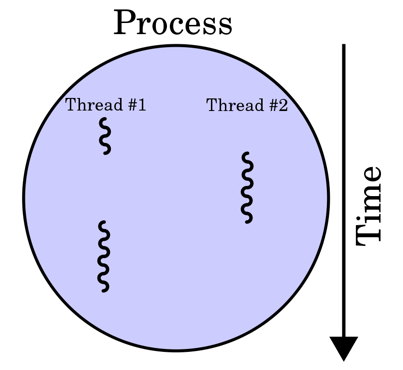
\includegraphics[width=0.4\linewidth]{images/midterm_2_solution_1.png}
            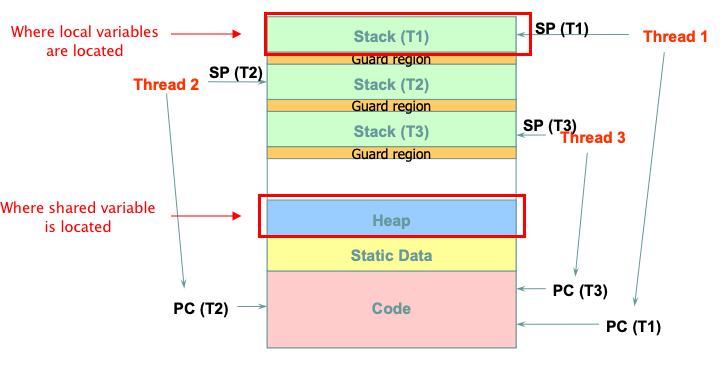
\includegraphics[width=\linewidth]{images/midterm_2_solution_2.png}
            \end{center}

            \item A thread is bound to a single process
            \item A process can have multiple threads
            \item Has two types
            \begin{itemize}
                \item \textbf{User-level Threads:}

                \begin{itemize}
                    \item Are implemented by users and kernel is not aware of the existence of these threads
                    \item Are represented by a program counter(PC), stack, registers and a small process control block
                    \item Are small and much faster than kernel level threads
                \end{itemize}
                \item \textbf{Kernel-level Threads:}

                \begin{itemize}
                    \item Are handled by the operating system directly
                    \item Thread management is done by the kernel
                    \item Are slower than user-level threads
                \end{itemize}
            \end{itemize}
        \end{itemize}

        \item \textbf{Process}

        \begin{itemize}
            \item Is a program in execution
            \item Is named by it's process ID or PID
            \item Can be described by the following states at any point in time

            \begin{itemize}
                \item Address Space
                \item CPU Registers
                \item Program Counter
                \item Stack Pointer
                \item I/O Information
            \end{itemize}

            (wait. this is PCB)

            \item Exists in one of many different \textbf{process states}, including

            \begin{enumerate}[1.]
                \item Running
                \item Ready to Run
                \item Blocked
            \end{enumerate}

            \bigskip

            \begin{itemize}
                \item Different events (Getting Scheduled, descheduled, or waiting for I/O)
                transitions one of these states to the other
            \end{itemize}

        \end{itemize}

        \item \textbf{Signals}

        \begin{itemize}
            \item Provides a way to communicate with the process
            \item Can cause job to stop, continue, or terminate
            \item Can be delivered to an application

            \begin{itemize}
                \item Stops the application from whatever its doing
                \item Runs Signal handler (some code in application to handle the signal)
                \item When finished, the process resumes previous behavior
            \end{itemize}
        \end{itemize}

        \item \textbf{Spinlock}
        \begin{itemize}
            \item Is the simplest lock to build
            \item Uses a lock variable

            \begin{itemize}
                \item 0 - (available/unlock/free)
                \item 1 - (acquired/locked/held)
            \end{itemize}

            \item Has two operations

            \begin{enumerate}[1.]
                \item \texttt{acquire()}

                \bigskip

                \begin{center}
                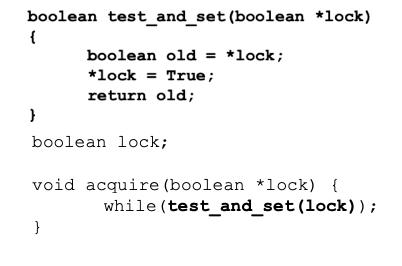
\includegraphics[width=0.7\linewidth]{images/midterm_2_solution_3.png}
                \end{center}

                \bigskip

                \item \texttt{release()}

                \bigskip

                \begin{center}
                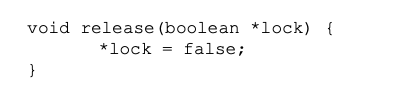
\includegraphics[width=0.7\linewidth]{images/midterm_2_solution_4.png}
                \end{center}

                \bigskip
            \end{enumerate}
            \item Allows a single thread to enter critical section at a time
            \item Spins using CPU cycles until the lock becomes available.
            \item May spin forever
        \end{itemize}

        \item \textbf{Scheduling policies}

        \begin{itemize}
            \item Are algorithms for allocating CPU resources to concurrent tasks
            deployed on (i.e., allocated to) a processor (i.e., computing resource)
            or a shared pool of processors $^{[5]}$
            \item Are sometimes called \textbf{Discipline}
            \item Covers the following algorithms in textbook

            \begin{itemize}
                \item \textbf{First In First Out}
                \item \textbf{Shortest Job First}
                \item \textbf{Shortest Time-to-completion First}
                \item \textbf{Round Robin}

                \begin{itemize}
                    \item Runs job for a \textbf{time slice} or \textbf{quantum}
                    \item Each job gets equal share of CPU time
                    \item Is clock-driven $^{[6]}$
                    \item Is starvation-free $^{[7]}$
                    \item \underline{Must} have the length of a time slice (\textbf{quantum}) as multiple of timer-interrupt period
                \end{itemize}

                \bigskip

                \begin{center}
                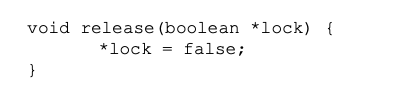
\includegraphics[width=0.7\linewidth]{images/midterm_2_solution_4.png}
                \end{center}
                \item \textbf{Multi-level Feedback Queue}
            \end{itemize}
        \end{itemize}

    \end{itemize}

    \bigskip

    \underline{\textbf{References}}

    \begin{enumerate}[1)]
        \item Coding Horror, Understanding User and Kernel Mode, \href{https://blog.codinghorror.com/understanding-user-and-kernel-mode/}{link}
        \item Kansas State University, Basics of How Operating Systems Work, \href{http://faculty.salina.k-state.edu/tim/ossg/Introduction/OSworking.html#:~:text=Interrupts%20are%20signals%20sent%20to,part%20of%20the%20operating%20system.&text=Hardware%20Interupts%20are%20generated%20by,some%20attention%20from%20the%20OS.}{link}
        \item Kansas State University, Glossary, \href{http://faculty.salina.k-state.edu/tim/ossg/glossary.html#term-context-switch}{link}
        \item Tutorials Point, User-level threads and Kernel-level threads, \href{https://www.tutorialspoint.com/user-level-threads-and-kernel-level-threads}{link}
        \item Science Direct, Scheduling Policy, \href{https://www.sciencedirect.com/topics/computer-science/scheduling-policy#:~:text=Scheduling%20policies%20are%20algorithms%20for,nature%20of%20applications%20%5B1%5D.}{link}
        \item Guru 99: What is CPU Scheduling?, \href{https://www.guru99.com/cpu-scheduling-algorithms.html#8}{link}
        \item Wikipedia: Round-robin Scheduling, \href{https://en.wikipedia.org/wiki/Round-robin_scheduling}{link}
    \end{enumerate}

    \item

    \begin{enumerate}[a)]
        \item Is a simple form of lock. It allows a single thread to enter ciritical section at a time. It
        spins using CPU cycles until lock becomes available. It uses variable \texttt{lock} with two values (0 for available, 1 for acquired) with
        operations \texttt{acquire()} and \texttt{release()}.
        \item Is a fraction of total turnaround time for a process. Is used by round-robin
        scheduling algorithm. A process under RR has equal parts of these. Furthermore, scheduling quantum
        assigned to a process to be multiples of timer-interrupt period

        \bigskip

        \begin{mdframed}
        \underline{\textbf{Correct Solution}}

        \bigskip

        \color{red}In a preemptive scheduler, this is the time alloted to a process before context-switching
        to another process\color{black}
        \end{mdframed}

        \item Is the programmatic way in which user requests for previleged service in operating system.
        On system call, the current process states (program counter, CPU register, kernal state) are saved,
        enters kernel mode, performs previleged operations such as reading the disk,
        executes return-from-trap instructions, and returns back to user mode and resumes
        the program with the attained result
    \end{enumerate}

    \bigskip

    \underline{\textbf{Notes}}

    \begin{itemize}
        \item \textbf{Response Time}
        \begin{itemize}
            \item \textbf{Formula} $T_{response} = T_{firstrun} - T_{arrival}$
            \item measures the interactive performance between users and the system
        \end{itemize}

        \item \textbf{Turnaround Time}

        \begin{itemize}
            \item \textbf{Formula} $T_{turnaround} = T_{completion} - T_{arrival}$
            \item measures the amount of time taken to complete a process
        \end{itemize}

        \item \textbf{System Call}

        \begin{itemize}
            \item Is the programmatic way in which a computer program requests a previleged service from the kernel of the operating system
            \item i.e. Reading from disk
            \item Steps

            \begin{enumerate}[1)]
                \item Setup \textbf{trap tables} on boot
                \item Execute system call
                \item Save \textit{Program Counter}, \textit{CPU registers}, \textit{kernal stack} (so process can resume after \textbf{return-from-trap}
                or \textbf{context switch})
                \item Switch from \textbf{user mode} to \textbf{kernel mode}
                \item Perform previleged operations
                \item Finish and execute \textbf{return-from-trap} instruction
                \item Return from \textbf{kernel mode} to \textbf{user mode} and resume user program
            \end{enumerate}
        \end{itemize}
    \end{itemize}

    \item

    \begin{enumerate}[a)]

        \item

        \texttt{(b)} is the only scheduling algorithm that causes starvation

        \underline{\textbf{Notes}}

        \begin{itemize}
            \item \textbf{Starvation}

            \begin{itemize}
                \item Is the problem that occurs when high priority processes keep
                executing and low priority processes get blocked for indefinite time $^{[1]}$
            \end{itemize}

            \item \textbf{Convoy Effect}

            \begin{itemize}
                \item Is the problem where number of relatively-short potential consumers
                of a resource get queued behind a heavy weight consumer

                \bigskip

                \begin{center}
                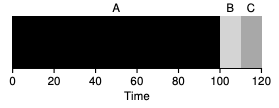
\includegraphics[width=0.7\linewidth]{images/midterm_2_solution_5.png}
                \end{center}
            \end{itemize}

            \item \textbf{First In First Out}

            \begin{itemize}
                \item Is the most basic scheduling algorithm
                \item Is vulnerable to \textbf{convoy effect}
                \item No \textbf{starvation} as long as every process eventually completes
            \end{itemize}

            \item \textbf{Shortest Job First}

            \begin{itemize}
                \item Improves average \textbf{turnaround time} given processes of uneven length
                \item Is a general scheduling principle useful in situation where turnaround time
                per process matters
                \item Is vulnerable to \textbf{convoy effect}

                \begin{center}
                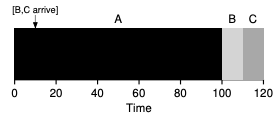
\includegraphics[width=0.7\linewidth]{images/midterm_2_solution_6.png}
                \end{center}

                \item Is vulnerable to \textbf{starvation}
                \begin{itemize}
                    \item When only short-term jobs come in while a long term job is in queue
                \end{itemize}
            \end{itemize}
            \item \textbf{Shortest Time-to-completion First}

            \begin{itemize}
                \item Addresses \textbf{convoy effect} in \textbf{Shortest Job First}
                \item Determines which of the remaining+new jobs has least time left, and
                schedule accordingly at \underline{any time}

                \bigskip

                \begin{center}
                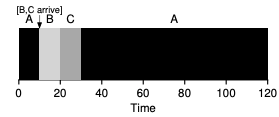
\includegraphics[width=0.7\linewidth]{images/midterm_2_solution_7.png}
                \end{center}

                \item Is vulnerable to \textbf{starvation}
                \begin{itemize}
                    \item When only short-term jobs come in while a long term job is in queue
                \end{itemize}

            \end{itemize}

            \item \textbf{Round Robin}

            \begin{itemize}
                \item Has good \textbf{response time} but terrible \textbf{turnaround time}
                \item Runs job for a \textbf{time slice} or \textbf{quantum}
                \item Each job gets equal share of CPU time
                \item Is clock-driven $^{[6]}$
                \item Is starvation-free $^{[7]}$
                \item \underline{Must} have the length of a time slice (\textbf{quantum}) as multiple of timer-interrupt period
            \end{itemize}

            \bigskip

            \begin{center}
            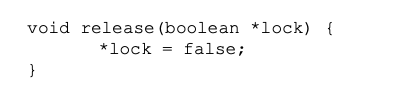
\includegraphics[width=0.7\linewidth]{images/midterm_2_solution_4.png}
            \end{center}
            \item \textbf{Multi-level Feedback Queue}

            \begin{itemize}
                \item Is the most well known approaches to shceduling
                \item Optimizes \textbf{turnaround time}, and minimizes \textbf{response time}
                \item Observees the execution of a job and priortizes accordingly without prior knowledge
                \item Rules

                \begin{itemize}
                    \item \textbf{Rule 1:} If Priority(A) $>$ Priority(B), A runs (B doesn't)
                    \item \textbf{Rule 2:} If Priority(A) $=$ Priority(B). A \& B run in round-robin
                    fashion using the time slice (quantum length) of the given queue
                    \item \textbf{Rule 3:} When a job enters the system, it is placed at the highest
                    priority(the top most queue)
                    \item \textbf{Rule 4:} Once a job uses up its time allotment at a given level
                    (regardless of how many times it has given up the CPU), its priority is reduced
                    (it moves down on queue)
                    \item \textbf{Rule 5:} After some time period S, move all the jobs in the system to the
                    topmost queue.
                \end{itemize}

                \bigskip

                \begin{center}
                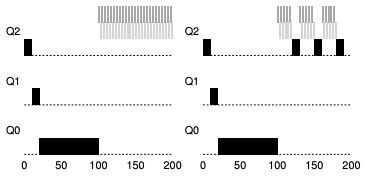
\includegraphics[width=0.7\linewidth]{images/midterm_2_solution_8.png}
                \end{center}
            \end{itemize}

        \end{itemize}

        \item

        Nothing. \texttt{pthread\_cond\_signal} unblocks at least one of the thread
        that are blocked on the specified condition variable \texttt{cond}. Since
        there are no other threads waiting on \texttt{cv1}, there are no threads to awake.

        \bigskip

        \underline{\textbf{Notes}}

        \begin{itemize}
            \item \textbf{Critical Section}

            \begin{itemize}
                \item Is a piece of code that accesses a \textit{shared} resource,
                \ul{usually a variable or data structure}
            \end{itemize}

            \item \textbf{Thread}

            \begin{itemize}
                \item Is a lightweight process that can be managed independently by a schdeduler $^{[4]}$
                \item Improves the application performance using parallelism. (e.g peach)

                \begin{center}
                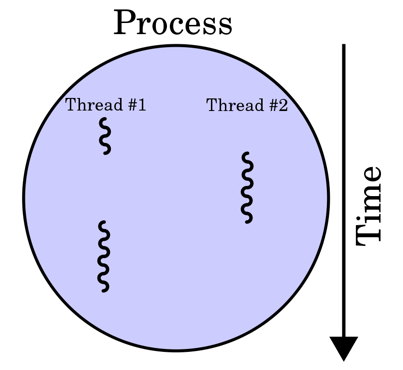
\includegraphics[width=0.4\linewidth]{images/midterm_2_solution_1.png}
                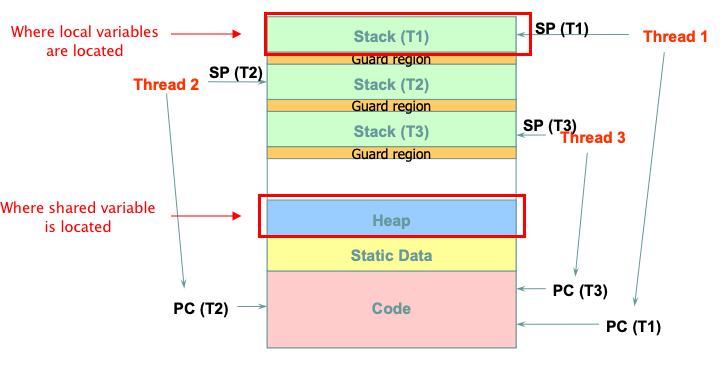
\includegraphics[width=\linewidth]{images/midterm_2_solution_2.png}
                \end{center}

                \item A thread is bound to a single process
                \item A process can have multiple threads
                \item Has two types
                \begin{itemize}
                    \item \textbf{User-level Threads:}

                    \begin{itemize}
                        \item Are implemented by users and kernel is not aware of the existence of these threads
                        \item Are represented by a program counter(PC), stack, registers and a small process control block
                        \item Are small and much faster than kernel level threads
                    \end{itemize}
                    \item \textbf{Kernel-level Threads:}

                    \begin{itemize}
                        \item Are handled by the operating system directly
                        \item Thread management is done by the kernel
                        \item Are slower than user-level threads
                    \end{itemize}
                \end{itemize}
            \end{itemize}

            \item \textbf{Thread API}

            \begin{itemize}

                \item \texttt{pthread\_cond\_wait}

                \begin{itemize}
                    \item Puts the calling thread to sleep (a blocked state)
                    \item Waits for some other thread to signal it
                \end{itemize}

                \bigskip

                \underline{\textbf{Example}}

                \begin{center}
                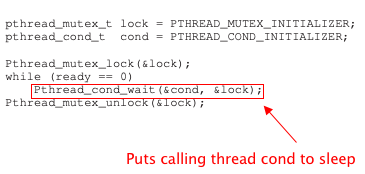
\includegraphics[width=0.7\linewidth]{images/midterm_2_solution_9.png}
                \end{center}

                \item \texttt{pthread\_cond\_signal}

                \begin{itemize}
                    \item Is used to \underline{unblocks at least one} of the threads that
                    are blocked on the specified condition variable cond
                \end{itemize}

                \bigskip

                \underline{\textbf{Example}}

                \begin{center}
                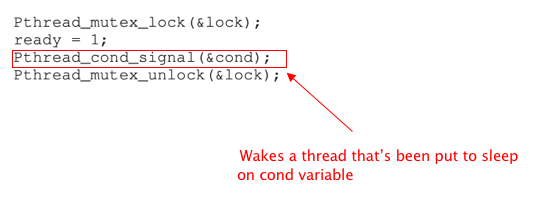
\includegraphics[width=0.8\linewidth]{images/midterm_2_solution_10.png}
                \end{center}

            \end{itemize}
        \end{itemize}

        \item

        Interrupt is a signals usually sent by external devices, normally I/O devices. It
        tells the CPU to stop the current process and execute appropriate part of
        the operating system.

        \bigskip

        System call is a programmatic way which a computer requests for previleged service
        from the kernel of the Operating System

        \bigskip

        \begin{mdframed}
        \underline{\textbf{Correct Solution}}

        \bigskip

        \color{red}Interrupt is a signals are sent by hardware (keyboardm mouse, etc.),
        or software (page fault, protection violation, system call)

        \bigskip

        System call is a strictly subset of software interrupts where a user program
        asks the OS to perform some previleged functionality on its behalf.

        \color{black}

        \end{mdframed}

        \bigskip

        \underline{\textbf{Notes}}

        \begin{itemize}
            \item \textbf{Interrupt}

            \begin{itemize}
                \item Are signals sent to the CPU by external devices, normally I/O devices.
                \item Tells the CPU to stop current process and execute appropriate part of the
                operating system
            \end{itemize}

            \item \textbf{System Call}

            \begin{itemize}
                \item Is the programmatic way in which a computer program requests a previleged service from the kernel of the operating system
            \end{itemize}
        \end{itemize}

        \item

        No. I don't agree. I tried to find the reasons regarding inner workings
        of kernel threads and user threads without success :(

        \item

        There are 3 additional processes in totoal. \texttt{fork()} produces a child
        process of \texttt{run\_itself} and one \texttt{exec()} produces a process for the
        command \texttt{ls -l} and the other \texttt{exec()} produces a process for
        command \texttt{cat /proc/cpuinfo}

        \bigskip

        \begin{mdframed}
        \underline{\textbf{Correct Solution}}

        \bigskip

        \color{red}Only 1 process, because the exec system call does not spawn any new processes\color{black}
        \end{mdframed}

    \end{enumerate}

    \item

    \begin{enumerate}[a)]

        \item

        I am not too sure on this one. My guess is that account one enters the critical section
        and while it's in critical section, account 2 switches context and goes to blocked state.

        \bigskip

        Then, account 1 need to wait for account 2. Thus, deadlock.
        \bigskip

        \begin{mdframed}
        \underline{\textbf{Correct Solution}}

        \bigskip

        \color{red}
        There are two scenarios.

        \begin{enumerate}[1.]
            \item When two accounts transfer at the same time.
            \begin{itemize}
                \item \texttt{user\_1} executes \texttt{transfer\_amount(user\_2, user\_1)}
                \item \texttt{user\_2} executes \texttt{transfer\_amount(user\_1, user\_2)}
                \item Each will acquire their own lock at \texttt{pthread\_mutex\_lock(a1->lock)}
                \item But because they are already locked \texttt{pthread\_mutex\_lock(a2->lock)} can't execute,
                thus deadlock
            \end{itemize}
            \item When performing self transfer

            \begin{itemize}
                \item \texttt{user\_1} executes \texttt{transfer\_amount(user\_1, user\_1)}
                \item \texttt{user\_1} will acquire own lock at \texttt{pthread\_mutex\_lock(a1->lock)}
                \item But because user\_1 is already locked, \texttt{pthread\_mutex\_lock(a2->lock)} can't execute,
                thus deadlock
            \end{itemize}
        \end{enumerate}
        \color{black}
        \end{mdframed}

        \bigskip

        \underline{\textbf{Notes}}

        \begin{itemize}
            \item \textbf{Semaphores}

            \begin{itemize}
                \item
            \end{itemize}

            \item \textbf{Livelock}

            \begin{itemize}
                \item Two or more threads reapeatedly attempting this code over and over (e.g acquiring lock), but progress is
                not being made (e.g acquiring lock)
                \item Solution: Add a random delay before trying again (decrease odd of livelock)
            \end{itemize}

            \item \textbf{Deadlock}

            \begin{center}
            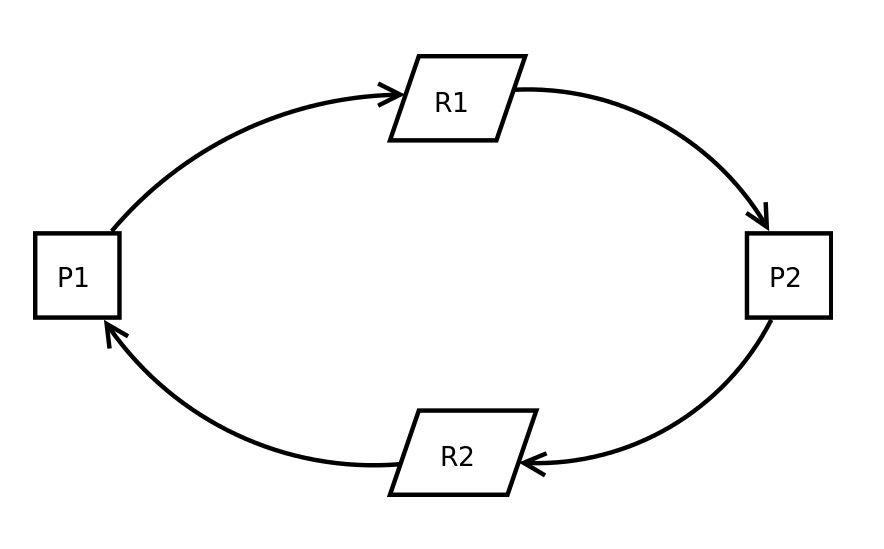
\includegraphics[width=0.6\linewidth]{images/midterm_2_solution_11.png}
            \end{center}

            \begin{itemize}
                \item Is a state in which each member of a group is waiting for
                another member including itself, to take action (e.g. releasing lock)
                \item Conditions for Deadlock (All four must be met)

                \begin{itemize}
                    \item \textbf{Mutual Exclusion}
                    \begin{itemize}
                        \item Occurs when threads claim exclusive control of resources that
                        they require (e.g. thread grabing a lock)
                    \end{itemize}
                    \item \textbf{Hold-and-wait}
                    \begin{itemize}
                        \item Occurs when threads hold resources allocated to them (e.g locks that they have already acquired)
                        while waiting for additional resources (e.g. locks that they wish to acquire)
                    \end{itemize}

                    \item \textbf{No Preemption}
                    \begin{itemize}
                        \item Occurs when resource cannot be forcibly removed from threads that are holding them
                    \end{itemize}
                    \item \textbf{Circular Wait}
                    \begin{itemize}
                        \item Occurs when there exists a circular chain of threads such that
                        each threads hold one or more resources (e.g. locks) that are being
                        requested by the next thread in the chain.
                    \end{itemize}
                \end{itemize}

                \bigskip

                \underline{\textbf{Example}}

                \begin{center}
                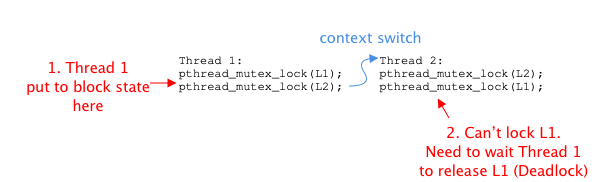
\includegraphics[width=0.9\linewidth]{images/midterm_2_solution_12.png}
                \end{center}

                \item Preventions

                \begin{itemize}
                    \item \textbf{Circular Wait}
                    \begin{itemize}
                        \item Write code such that circular wait is never induced
                        \item Is the most practical prevention technique
                        \item Requires deep understanding of the code base
                        \item \textbf{Total Ordering} (Most starightforward)

                        \bigskip

                        \underline{\textbf{Example}}

                        \bigskip

                        Given two locks in the system (\texttt{L1} and \texttt{L2}), always
                        acuiqure \texttt{L1} before \texttt{L2}

                        \bigskip

                        \item \textbf{Partial Ordering} (Applied to complex systems)

                        \bigskip

                        \underline{\textbf{Example}}

                        \bigskip

                        Memory mapping code in Linux (has then different groups).

                        \bigskip

                        (Simple) \texttt{i\_mutex} before \texttt{i\_mmap\_mutex}

                        \bigskip

                        (More complex) \texttt{i\_mmap\_mutex} before \texttt{private\_lock}
                        before \texttt{swap\_lock} before \texttt{mapping->tree\_lock}

                    \end{itemize}

                    \item \textbf{Hold-and-wait}
                    \begin{itemize}
                        \item Can be avoided by acquiring all locks at once
                        \item Can be problematic
                        \item Must know which lock must be held and acquire ahead of time
                        \item Is likely to decrease concurrency (since all need to be acquired over their needs)

                        \bigskip

                        \underline{\textbf{Example}}

                        \bigskip

                        \begin{center}
                        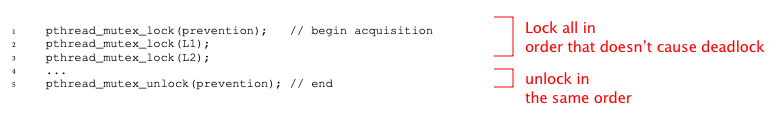
\includegraphics[width=\linewidth]{images/midterm_2_solution_13.png}
                        \end{center}
                    \end{itemize}

                    \item \textbf{No Preemption}
                    \begin{itemize}
                        \item Can be avoided by adding code that force unlock if not available

                        \begin{center}
                        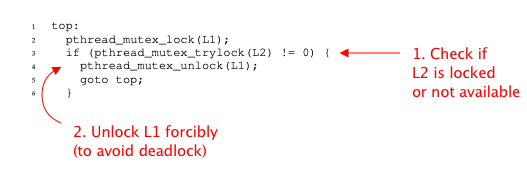
\includegraphics[width=0.8\linewidth]{images/midterm_2_solution_14.png}
                        \end{center}

                        \item \texttt{pthread\_mutex\_trylock} tries to lock the speicied mutex.
                        \item \texttt{pthread\_mutex\_trylock} returns 0 if lock is available
                        \item \texttt{pthread\_mutex\_trylock} returns the following error if occupied

                        \bigskip

                        \quad \texttt{EBUSY} - Mutex is already locked

                        \bigskip

                        \quad \texttt{EINVAL} - Is not initialized mutex

                        \bigskip

                        \quad \texttt{EFAULT} - Is in valid pointer

                        \item May result in \textbf{live lock}
                    \end{itemize}

                    \item \textbf{Mutual Exclusion}
                    \begin{itemize}
                        \item Idea: Avoid the mutual exclusion at all
                        \item Use \textbf{lock-free}/\textbf{wait-free} approach:
                        building data structures in a manner that does not require explicit locking
                        using hardware instructions

                        \bigskip

                        \underline{\textbf{Example}}

                        \bigskip

                        \begin{center}
                        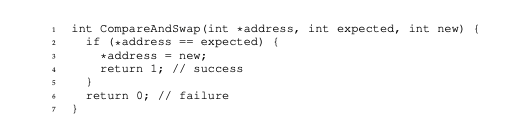
\includegraphics[width=\linewidth]{images/midterm_2_solution_15.png}
                        \end{center}

                    \end{itemize}
                \end{itemize}

                \item Avoidance

                \begin{itemize}
                    \item \textbf{Banker's Algorithm}
                \end{itemize}
            \end{itemize}
        \end{itemize}
    \end{enumerate}

\end{enumerate}

\end{document}